\begin{figure}[t]
  \centering
  \pgfdeclarelayer{background}   % layer with the synthesizer rectangle
  \pgfsetlayers{background,main} % background behind main
  
  
    \begin{tikzpicture}[%
  auto,
  trim left=(user), trim right=(user)
] %, trim right=(spec)]
  \sffamily
  
  \node[square] (verifier) {Verifier};

  \node[square] (enumerator) [above=1 of verifier] {Enumerator};

  \node[nosquare] (DSL) [above=0.3 of enumerator] {DSL};
  
  \node [nosquare, black, font=\bf\sffamily] (io_examples) [left=1.5 of verifier, align=center] {I/O\\examples};
  
  \node[square] (distinguisher) [right=1.5 of verifier, align=center]
  {Distinguisher};
  
  \node (user) [below right=.7 and 0.2 of verifier]
  {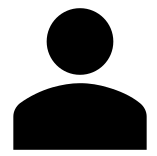
\includegraphics[width=1cm]{pictures/user2.png}};
  
  \node[nosquare] (desired) [black, font=\bf\sffamily, right=1.5 of distinguisher, align=center] {Desired\\Program};

  
  \draw [arrow, bend right=45] (enumerator) to  node[align=center, left] (candidate) {candidate\\program} (verifier);

  \draw [arrow, bend right=45] (verifier) to node[align=center, right]  (failure) {reason\\of failure}  (enumerator);

  \draw [arrow] (DSL) to (enumerator);
  
  \draw [arrow] (io_examples) to (verifier);

  \draw [arrow] (distinguisher)  to [align=left, right] node (unsat) {} (desired);
  
  \draw [arrow] (verifier) to node [align=center, below] (p1p2) {2 correct\\programs}
  (distinguisher);
  
  \draw [arrow,  bend left=30] (user.170) to node [left=.3, align=center, near start] (new_io_example) {new I/O\\example} (verifier.south);
  
  \draw [arrow, bend left=30] (distinguisher.south) to node [right=.2, align=center, near end] (dist_input) {new\\input} (user.10);
  

  
  %\draw [arrow] (distinguisher.west) to node [align=right, below=.3] (dist_input) {%
  %  distinguishing input%
  %} (user);

  
  \begin{pgfonlayer}{background}
    \path let \p1=(enumerator.west),
              \p2=(DSL.north)
    in
      coordinate (topleftcorner) at (\x1, \y2);
      
    \path let \p1=(distinguisher.east),
              \p2=(p1p2.south)
    in
      coordinate (bottomrightcorner) at (\x1, \y2);
      
    \path let \p1=(topleftcorner),
              \p2=(bottomrightcorner)
    in
      coordinate (toprightcorner) at (\x2,\y1);
    
    % gre grey square representing synth's domain
    \draw[enclosing_square]
      ($(topleftcorner)+(-1.2,.1)$) rectangle
      ($(bottomrightcorner)+(1,-.1)$);
    
    \node[synth_node, anchor=north west] (synthtext) at ($(toprightcorner)+(-0.9,0)$) {Synthesizer};
  \end{pgfonlayer}

  \end{tikzpicture}

  \caption{Interactive synthesis algorithm.}
  \label{fig:interactive-synthesis}
\end{figure}